% Options for packages loaded elsewhere
\PassOptionsToPackage{unicode}{hyperref}
\PassOptionsToPackage{hyphens}{url}
%
\documentclass[
  man, fleqn, noextraspace]{apa6}
\usepackage{lmodern}
\usepackage{amssymb,amsmath}
\usepackage{ifxetex,ifluatex}
\ifnum 0\ifxetex 1\fi\ifluatex 1\fi=0 % if pdftex
  \usepackage[T1]{fontenc}
  \usepackage[utf8]{inputenc}
  \usepackage{textcomp} % provide euro and other symbols
\else % if luatex or xetex
  \usepackage{unicode-math}
  \defaultfontfeatures{Scale=MatchLowercase}
  \defaultfontfeatures[\rmfamily]{Ligatures=TeX,Scale=1}
\fi
% Use upquote if available, for straight quotes in verbatim environments
\IfFileExists{upquote.sty}{\usepackage{upquote}}{}
\IfFileExists{microtype.sty}{% use microtype if available
  \usepackage[]{microtype}
  \UseMicrotypeSet[protrusion]{basicmath} % disable protrusion for tt fonts
}{}
\makeatletter
\@ifundefined{KOMAClassName}{% if non-KOMA class
  \IfFileExists{parskip.sty}{%
    \usepackage{parskip}
  }{% else
    \setlength{\parindent}{0pt}
    \setlength{\parskip}{6pt plus 2pt minus 1pt}}
}{% if KOMA class
  \KOMAoptions{parskip=half}}
\makeatother
\usepackage{xcolor}
\IfFileExists{xurl.sty}{\usepackage{xurl}}{} % add URL line breaks if available
\IfFileExists{bookmark.sty}{\usepackage{bookmark}}{\usepackage{hyperref}}
\hypersetup{
  pdftitle={Differences in Stress Response by Ethnicity},
  pdfauthor={Ruby Cuellar, Ellen Huang, \& Angela Lee},
  pdfkeywords={sleep, stress, ethnicity},
  hidelinks,
  pdfcreator={LaTeX via pandoc}}
\urlstyle{same} % disable monospaced font for URLs
\usepackage{graphicx,grffile}
\makeatletter
\def\maxwidth{\ifdim\Gin@nat@width>\linewidth\linewidth\else\Gin@nat@width\fi}
\def\maxheight{\ifdim\Gin@nat@height>\textheight\textheight\else\Gin@nat@height\fi}
\makeatother
% Scale images if necessary, so that they will not overflow the page
% margins by default, and it is still possible to overwrite the defaults
% using explicit options in \includegraphics[width, height, ...]{}
\setkeys{Gin}{width=\maxwidth,height=\maxheight,keepaspectratio}
% Set default figure placement to htbp
\makeatletter
\def\fps@figure{htbp}
\makeatother
\setlength{\emergencystretch}{3em} % prevent overfull lines
\providecommand{\tightlist}{%
  \setlength{\itemsep}{0pt}\setlength{\parskip}{0pt}}
\setcounter{secnumdepth}{-\maxdimen} % remove section numbering
\shorttitle{DIFFERENCESINSTRESS}
\affiliation{
\vspace{0.5cm}
\textsuperscript{1} University of Oregon}
\keywords{sleep, stress, ethnicity}
\usepackage{csquotes}
\usepackage{upgreek}
\captionsetup{font=singlespacing,justification=justified}

\usepackage{longtable}
\usepackage{lscape}
\usepackage{multirow}
\usepackage{tabularx}
\usepackage[flushleft]{threeparttable}
\usepackage{threeparttablex}

\newenvironment{lltable}{\begin{landscape}\begin{center}\begin{ThreePartTable}}{\end{ThreePartTable}\end{center}\end{landscape}}

\makeatletter
\newcommand\LastLTentrywidth{1em}
\newlength\longtablewidth
\setlength{\longtablewidth}{1in}
\newcommand{\getlongtablewidth}{\begingroup \ifcsname LT@\roman{LT@tables}\endcsname \global\longtablewidth=0pt \renewcommand{\LT@entry}[2]{\global\advance\longtablewidth by ##2\relax\gdef\LastLTentrywidth{##2}}\@nameuse{LT@\roman{LT@tables}} \fi \endgroup}


\DeclareDelayedFloatFlavor{ThreePartTable}{table}
\DeclareDelayedFloatFlavor{lltable}{table}
\DeclareDelayedFloatFlavor*{longtable}{table}
\makeatletter
\renewcommand{\efloat@iwrite}[1]{\immediate\expandafter\protected@write\csname efloat@post#1\endcsname{}}
\makeatother
\raggedbottom
\setlength{\parskip}{0pt}

\title{Differences in Stress Response by Ethnicity}
\author{Ruby Cuellar\textsuperscript{1}, Ellen Huang\textsuperscript{1}, \& Angela Lee\textsuperscript{1}}
\date{}

\authornote{

Correspondence concerning this article should be addressed to Ruby Cuellar, Department of Psychology, 1227 University of Oregon, Eugene, OR 97403. E-mail: \href{mailto:rcuellar@uoregon.edu}{\nolinkurl{rcuellar@uoregon.edu}}}

\abstract{
Sleep disturbances are widely prevalent and represent a significant health problem in the general population. Minorities sleep a significantly less amount of time than Whites. Given that Latinos are the largest ethnic minority in the U.S., it is important to understand patterns and correlations of sleep characteristics in this population. The overall objective of this study was to examine the association between self-reported sleep characteristics and stress response between Mexican American and White college students. For this purpose, a study was designed where stress response would be measured by changes in heart rate and changes in heart rate variability following a stressful lab task with 133 undergraduate students. Sleep was measured using ten consecutive days of sleep diaries preceding the lab stress test. It was hypothesized that poor sleep would be associated with a greater stress response. It was also hypothesized that Mexican Americans would report less sleep duration compared to White Americans. Given these predictions, it was expected that Mexican Americans would exhibit higher levels of stress response, compared to Whites. Results indicated no significant sleep differences between Mexican Americans and Whites. However, the results demonstrated ethnic difference in stress response, where White college students seem to respond more negatively to the stressor than to Mexican American college students. Ultimately, the present study was able to fill a gap in the literature and determine whether any sleep differences exist in a sample of equally represented Mexican American and White. This study in particular addressed the low representation of Latinos in previous studies and the college population, as well as possible culture and ethnic related factors in psychophysiology.


}

\begin{document}
\maketitle

\hypertarget{introduction}{%
\section{Introduction}\label{introduction}}

Sleep is essential for daily functioning, health, and optimal development. Disturbed or poor sleep has the potential to impair levels of stress the following day (Garde, Albertsen, Persson, Hansen, \& Rugulies, 2012), as well modulates numerous physiological processes, including stress response and recovery. Such findings suggest that adequate sleep plays an important role in how individuals respond to stress. High stress due to lack of sleep causes a dysregulation to the autonomic nervous system, specifically the sympathetic nervous system (SNS) (Mellman, Bell, Abu-Bader, \& Kobayashi, 2018). Hyperactivity of the SNS has been long recognized as a major risk of the relationship between stress and cardiovascular disease (Cohen, Janicki-Deverts, \& Miller, 2007). On the other hand, the parasympathetic nervous system (PNS) regulates the SNS activity to bring the ANS back to homeostasis. Sleep is one mechanism by which PNS offsets SNS activity (Mellman et al., 2018). Consequently, insufficient sleep due to stress is a risk factor for a variety of physical and psychological problems, such as cardiovascular disease, obesity, diabetes, depression, and anxiety (Fuligni \& Hardway, 2006).

Adolescents are at high risk for insufficient sleep (Tsai \& Li, 2004), particularly as they transition into college (Doane, Gress-Smith, \& Breitenstein, 2015; Sladek \& Doane, 2015). Many university students meet the requirements for partial sleep deprivation (i.e.~less than 5 hours of sleep in a 24-hour period) and delayed sleep phase syndromes (difficulty falling asleep and waking up) (Galambos, Dalton, \& Maggs, 2009). The complex demands on college students, coupled with the risk created by insufficient sleep, makes understanding the link between sleep and stress response and recovery a priority. Additionally, college is an opportune time for interventions, which set the stage for long-term behavioral health.

The United States population and college student body is growing increasingly diverse. Latinos are the largest ethnic minority group in the U.S, with Mexican Americans being the largest subgroup, and are expected to comprise approximately 30\% of the population by 2050. Latinos face health disparities compared to non-Latino Whites, such as higher rates of cardiovascular heart disease (Hunt et al., 2003), obesity, and diabetes, all three which have been linked to sleep problems in other populations (Howrey, Peek, Raji, Ray, \& Ottenbacher, 2012). Additionally, co-existing sleep problems such as sleep apnea or sleep deprivation could also impact the management of diabetes, obesity, and other sleep related conditions. This data suggests a potential bi-directional effect between sleep and well-being and highlights the importance of understanding mechanisms that might contribute to poor health, such as insufficient sleep and impaired stress response and recovery.

There is a small body of evidence that Latinos are at-risk of insufficient sleep (Jean-Louis, Kripke, Ancoli-Israel, Klauber, \& Sepulveda, 2000; Loredo et al., 2010). Some data suggests that the prevalence of sleep problems and predictors of sleep duration are different in Latinos versus Whites. Such differences include differences in sleep architecture, such that Latino children experience less deep sleep than White children (Loredo et al., 2010). Additionally, Latinos have higher risk of insomnia and hyperinsomnia, and differences in environmental determinants; specifically, Latino children are more likely to live in environments that disturb their sleep. Much of the limitations in knowledge stem from under-representation of Latinos in sleep research (Jean-Louis et al., 2000; Knutson, 2010; Krueger \& Friedman, 2009; Pedraza, Al Snih, Ottenbacher, Markides, \& Raji, 2012). Importantly, no studies have examined the link between sleep and stress response or recovery among Latino college students in a prospective, quasi-experimental study.

This study aims to elucidate the role of Latino ethnicity in the link between sleep and stress response and recovery among college students by comparing equivalent size groups of Latino and non-Latino white young adults. Identifying variation in the link between sleep and stress response and recovery by ethnicity would stimulate the development of culturally sensitive prevention and intervention programs. It is hypothesized that being Latino will influence the strength of the relationship between sleep duration and quality and stress response and recovery. Specifically, it is expected that Latinos will experience greater stress response and diminished stress recovery compared to Whites. Support for this hypothesis would provide a framework for addressing health disparities.

\hypertarget{methods}{%
\section{Methods}\label{methods}}

\hypertarget{design}{%
\subsection{Design}\label{design}}

This is a quasi-experimental study in which equivalent groups of Latino and non-Latino white college students were exposed to a stress manipulation to observe their physiological stress response and recovery. Self-reported sleep was measured prospectively for 10 days leading up to the stress induction.

\hypertarget{participants}{%
\subsection{Participants}\label{participants}}

A sample of 133 undergraduate students (53\% Mexican American, 47\% Whites) were recruited from a Human Participant Pool (HPP) or summer classes at a university in Southern California. Inclusion criteria required participants to be enrolled college students, be 18-24 years old, be proficient in English and identify themselves as being Mexican American or White. The requirement of being Mexican American was to provide homogeneity within the diverse Latin American culture; Mexican American was chosen because it is the largest country of origin among U.S. Latinos (Loredo et al., 2010). Participants who reported any medical condition that could be exacerbated from stress, reported having an extreme fear of public speaking, had a current psychiatric diagnosis related to stress, or an inability to cope with stress were excluded from the study.

\hypertarget{measures}{%
\subsection{Measures}\label{measures}}

\hypertarget{descriptive-measures}{%
\subsubsection{Descriptive Measures}\label{descriptive-measures}}

\emph{Demographics.} Participants were asked demographic questions about race/ethnicity, generation status, gender, and age.

\hypertarget{sleep-characteristics}{%
\subsubsection{Sleep Characteristics}\label{sleep-characteristics}}

\emph{Daily Diary.} Sleep patterns were monitored with an online sleep diary. Students were instructed to complete a three-minute survey every night before bed for ten consecutive nights. The daily diaries consisted of questions pertaining to the prior night's sleep (adapted from (Fuligni, Tsai, Krull, \& Gonzales, 2015)). The diaries assessed the participants sleep duration and sleep quality. A mean for both sleep domains was calculated from the daily diary surveys.

\hypertarget{stress-induction}{%
\subsubsection{Stress Induction}\label{stress-induction}}

\emph{Trier Social Stress Task.} The Trier Social Stress Test (TSST), adapted by Yim, Quas, Rush, Granger, and Skoluda (2015) was used to induce stress. During the TSST, the participant entered a room where one male and one female judge were waiting. The participants were instructed to deliver a 5-minute speech, followed by mental arithmetic in front of the judges while being videotaped. If at any moment they stopped, they were instructed to continue with the task until the five minutes were up (only two reminders were allowed). If they stopped again or remained silent for 15 seconds, the judge would instruct them to continue standing for the remainder of the time.

\hypertarget{stress-response-and-recovery.}{%
\subsubsection{Stress Response and Recovery.}\label{stress-response-and-recovery.}}

\emph{Autonomic stress response.} The study assessed the participants' autonomic response to stress by measuring heart rate, specifically mean beats per minute (BPM) and heart rate variability (HRV), using Biopac wireless Electrocardiogram (ECG) equipment and Bionomadix software. Participants were connected to the Biopac system using wireless Electrocardiogram (ECG) equipment five minutes before the initiation of the TSST in order to get a baseline measure and remained connected until the completion of the study. Three mean heart rate values were extracted for each participant for each measure of heart rate. In other words, 5 minutes were extracted from baseline (T1), 15 minutes during the TSST (T2), and 35-min during recovery (T3) for both BPM and HRV. Stress reactivity corresponds to the change score from baseline to TSST (T1 and T2), while stress recovery corresponds to change scores from TSST and recovery (T2 and T3).

\hypertarget{procedure}{%
\subsection{Procedure}\label{procedure}}

The present study consisted of two sessions with a ten-day, daily assessment in-between the sessions. During Session 1, participants provided consent to the study. They were then screened to see if they met the criteria required to participate. Qualified participants were asked to fill out their demographic information and given instructions for the at-home portion that involved the daily diaries. Lastly, participants were scheduled for Session 2. Session 2 was scheduled about two weeks after the initial visit. During the at home portion of this study, participants were instructed to fill out an online survey about their daily sleeping habits before bed, every night, for ten consecutive days. Participants automatically received an email at 6 am the following morning reminding them to complete the diary in case they had forgotten. Participants were told to ignore the second email if the diary had been completed the night before. Session 2 was the final stage of the study. Upon arrival participants were introduced to the task environment, and hooked up to the wireless ECG equipment. Participants were asked to relax and breathe normally for five minutes while baseline heart rate was measured. Following the baseline, participants were briefed on the speech task. They were given three minutes to prepare a 5-minute mock interview to deliver in front of a panel that they believed were judging their performance. Following the speech, participants were instructed to perform some basic mental arithmetic -- serial subtraction -- for 5 minutes. At the conclusion of both tasks, the 35-minute recovery period began. Participants were given a questionnaire packet to complete as well as an eleventh daily diary to control for the previous night's sleep. Upon completing the questionnaires, participants were invited to read neutral material and relax in the pre-task room for the remainder of the time. At the conclusion of the 35 minutes, the participants were unhooked from the Biopac equipment, were debriefed on the study, and supplied a referral for counseling services at the university.

\hypertarget{analytic-approach}{%
\subsection{Analytic Approach}\label{analytic-approach}}

Following data collection and data entry, all data were checked in order to assess for normality, skewness, kurtosis, missing data, and outliers. Winsorizing was used to correct for normality and to address outliers. Given the high attrition rate of this study, 133 participants completed daily diaries; however, not all participants completed the second session. Due to this and uninterruptible heart rate data, the final sample was reduced to 107. In order to account for the participants' sleep the night prior to the stressors, an eleventh dairy was controlled for. However, this block was removed from the analysis because the eleventh diary did not significantly contribute to the overall model. Participants' stress reactivity (changes in heart rate and heart rate variability) was regressed onto their self-reported measures of sleep duration and ethnicity and the interaction between them. We used R Version 3.6.1 (R Core Team, 2019) for all our analyses.

\hypertarget{results}{%
\section{Results}\label{results}}

Consistent with the demographics of the university, participants were predominantly female (77\%). When analyzing heart rate, both BPM and HRV demonstrated normal stress response. Two one-way analysis of variances (ANOVAs) were conducted to determine difference among the three time points in BPM and HRV. Means and standard deviations across participants are displayed in Table 1. The first ANOVA demonstrated significant variation among time points in HRV \emph{F}(2,3) = 15.87, \emph{p} = .03. A post hoc Tukey test revealed that the difference lies between TSST ( \emph{M} = 27.92, \emph{SD} = 14.83) and recovery ( \emph{M} = 50.83, \emph{SD} = 29.85). The second ANOVA test also yielded significant variation among the three time points in BPM \emph{F}(2,3) = 100.7, \emph{p} = .002, a post hoc Tukey test revealed the differences between time points were at Baseline ( \emph{M} = 82.08, \emph{SD} = 13.31) and TSST ( \emph{M} = 97.56, \emph{SD} = 15.69) and TSST and recovery ( \emph{M} = 76.93, \emph{SD} = 10.62).
When examining ethnicity as a moderator for the relationship between sleep domains (quality and duration) and stress response (reactivity and recovery) for both measures of heart rate (BPM and HRV), eight moderation analyses were conducted (See figures 1 and 2). Results demonstrated no significant interactions between sleep and ethnicity for any moderation model. However, main effects of ethnicity were found for both sleep domains and both stress reactivity and stress recovery when measured by mean BPM. Therefore, the interaction terms were dropped and simple regression was conducted to examine the association between ethnicity and stress reactivity and recovery. Regression analysis results indicate that White participants were more likely to experience an increase in heart rate during stressor, \emph{F}(1, 113) = 4.56, \emph{p} = 0.03, \emph{R\textsuperscript{2}} = .04, and more likely to recover faster from the stressor, \emph{F}(1, 113) = 7.11, \emph{p} = 0.009, \emph{R\textsuperscript{2}} = .06, than Mexican American participants.

\hypertarget{discussion}{%
\section{Discussion}\label{discussion}}

The aim of this study was to examine the role of Latino ethnicity in the relationship between sleep and stress reactivity/recovery among college students. Our data suggests there are no ethnic differences in sleep duration or quality. However, the results did reveal ethnicity as a main effect on stress response. Specially, ethnicity was associated with how one reacts to a stressor and how rapidly they recover from such stressor. These findings suggest that White college students tend to respond faster to the stressor, or have a higher reactivity to the stressor, compared to Mexican American college student. The results also suggest that White college students recover from the stressor faster than do Mexican American students. Overall, these findings indicate that stress response (i.e.~reactivity and recovery) are different between White and Mexican American college students.

\hypertarget{sleep-differences-based-on-ethnicity}{%
\subsection{Sleep Differences Based on Ethnicity}\label{sleep-differences-based-on-ethnicity}}

When examining sleep differences between two ethnic groups, Mexican Americans and Caucasian, this study was unable to replicate the findings that sleep problems (e.g.~less sleep time, poor sleep quality) are more common among nonwhite minorities (Bixler, Vgontzas, Lin, Vela-Bueno, \& Kales, 2002; Jean-Louis et al., 2000). However, it should be noted that other studies have found the opposite, that minorities sleep more, to be true (Hale \& Do, 2007) . The two studies that found differences in sleep based on ethnicity had a sample size comprised of multiple ethnic minority backgrounds and some that did not include Latinos at all (Bixler et al., 2002; Jean-Louis et al., 2000). Additionally, the studies that looked at Latinos, specifically Mexican Americans have found conflicting results. Hale and Do (2007) found that Mexican Americans were more likely to be long sleepers (sleeping more than nine hours) compared to Caucasians; however Mexican Americans comprised only 4\% of the entire sample, as opposed to their Caucasian counterparts who accounted for 79\% of the entire sample. These studies have yielded conflicting results that serve as evidence for the importance of equally represented minority groups.
The present study was able to fill a gap in the literature and determine whether any sleep differences exist in a sample of equally represented Mexican American and Caucasian.

This study in particular addressed the low representation of Latinos in previous studies and the college population, as college students are known to experience lifestyle changes that create precipitating factors that can affect both sleep and stress (e.g.~erratic schedules, all-nighters, high-stress period like final exams; Lund, Reider, Whiting, \& Prichard, 2010). In fact, many college students meet criteria for partial sleep deprivation (e.g., sleeping \textless{} 5 hr. in 24 hrs; Galambos et al., 2009)). This transition process can take a toll on college students' overall health, and most importantly, it can be detrimental to their sleep behaviors. Results of this study indicated no significant differences between Mexican American and Caucasian college students in the amount of mean sleep duration or the quality of sleep. Mexican Americans slept on average, 20 minutes less than their Caucasian counterparts did, but this relationship was not significant. One reason behind these findings could be the fact that college students in general report routinely getting insufficient sleep (Sladek \& Doane, 2015). Any possible ethnic differences could have been overpowered due to the common characteristic of being a college student and the overall poor sleep of college students.

\hypertarget{ethnicity-as-a-moderator-for-sleep}{%
\subsection{Ethnicity as a Moderator for Sleep}\label{ethnicity-as-a-moderator-for-sleep}}

When examining ethnicity as moderator for the relationship between sleep and stress, the results were not significant. The interaction between sleep and ethnicity did not predict sleep response. However, ethnicity stood out as a main effect in the models examining sleep duration and sleep quality as predictors of stress response measured by BPM. The interaction term was dropped and a simple regression was used to examine the association between ethnicity and stress reactivity and stress recovery. The results suggest that ethnicity is associated with stress reactivity and recovery when measured by BPM. More specifically, being a white college student demonstrated a higher stress reactivity and faster stress recovery. These results suggest that stress response is different between Mexican American and White college students. More research is needed on Mexican Americans and Whites in order to establish differences in sleeping behaviors and how they are linked to stress. More specifically, what factors are contributing to differences in stress response between the two groups.

One possible explanation for these results is The Hispanic Health Paradox, the epidemiological phenomenon documenting better health and lower mortality of Hispanics/Latinos compared to non-Hispanic Whites despite being more vulnerable group (Ruiz, Sbarra, \& Steffen, 2018). Like other racial and ethnic minorities, Latinos tend to experience a disproportionate burden of socioeconomic (SES) and experience marginalization/discrimination that can cause psychosocial and physical health challenges (Ruiz et al., 2018). Similarly, Latinos suffer from significant economic disparities such as lower wage earning, lower median household income, and a poverty rate twice as high of that of Whites. These SES disparities in turn contribute to the significant social stress exposure including living in more disadvantaged neighborhoods (i.e.~higher crime neighborhoods, fewer neighborhood resources, poor education, and lower access to quality healthcare). However, despite these detriments, Hispanic/Latinos experience better health and have higher life expectancy than Whites.

It is possible that Latinos do not experience the same response to stress because they are more resilient than Whites (Ruiz, Hamann, Mehl, \& O'Connor, 2016; Ruiz et al., 2018). This Sociocultural Hypothesis is currently the dominant hypothesis used to explain the broad health advantages seen in Hispanic/Latinos and it focuses on cultural factors facilitating health-promoting social processes. This hypothesis suggests that collectivism facilitates social integration and support with downstream health benefits (Ruiz et al., 2016, 2018). Most importantly, social integration is a significant predictor of health, including disease morbidity and mortality and serves as a key health promoting process which affect health through social mechanisms. Despite the Hispanics/Latinos being a high-risk population, it is possible that they experience relatively less stress than other groups. In other words, their perception of a stressful stimulus is critical to the affective and physiological cascade believed to impact health.

\hypertarget{strengths-and-limitations}{%
\subsection{Strengths and Limitations}\label{strengths-and-limitations}}

This study was the first to examine ethnicity as a potential moderator for the relationship between sleep and stress and is one of the few studies that focus on sleep in Mexican Americans. A strength of this study was the use of two physiological measures to examine stress reactivity and recovery. This study used both heart rate (BPM) and heart rate variability (HRV) to accurately capture stress response. While the HRV data did not reveal significant results, we are to examine both sympathetic and parasympathetic responses. Additionally, the use of daily diaries can be seen as both a strength and limitation. Daily diaries strengthened the study because they record subjects' sleep patterns across several days and do not introduce errors of estimation related to retrospective recall as compared to a questionnaire that has participants recall their sleep in the past two weeks. However, they are still a subjective method of collecting sleep behaviors.

There are also limitations to the study, for example the sample of the study. Although this study aimed to find ethnic difference in sleep and stress, these effects may have been missed due to focusing on college students. Sleep problems are very prominent in the general population; however, college students are recognized as a population particularly affected by them. In fact, about 70\% of college students report regular sleep difficulties(Buboltz Jr, Brown, \& Soper, 2001). One study examined the effects of sleep deprivation on stress and found that in a sample of 22-50 year olds, sleep deprivation was linked to higher levels of stress when exposed to the TSST (Minkel et al., 2014). As this analysis focused on college students, a population known to experience the most sleep disturbances and stress, possible sleep differences between these two ethnicities may not have been captured.

\hypertarget{conclusion}{%
\subsection{Conclusion}\label{conclusion}}

The present study revealed considerable homogeneity in college student sleep, suggesting that college provides a unique culture that over-rides ethnic differences in sleep previously found in non-college samples. Ethnicity was associated with stress response, suggesting a difference in stress response between the two groups. A larger sample size would provide sufficient power to detect what might be a small but clinically significant effect. Additionally, examining social support, culture identity, acculturation status, and perceived stress can help future research and support the hypothesis that culture and ethnic factors play a significant role in psychophysiological research.

\newpage

\begin{table}[tbp]
\begin{center}
\begin{threeparttable}
\caption{\label{tab:unnamed-chunk-1}Mean scores and standard deviations across timepoints}
\begin{tabular}{lllll}
\toprule
 & \multicolumn{2}{c}{Mean} & \multicolumn{2}{c}{SD} \\
\cmidrule(r){2-3} \cmidrule(r){4-5}
Time Point & BPM & HRV & BPM & HRV\\
\midrule
baseline & 82.08 & 41.96 & 13.31 & 23.99\\
tsst & 97.56 & 27.92 & 15.69 & 14.83\\
recovery & 76.93 & 50.83 & 10.62 & 29.85\\
\bottomrule
\end{tabular}
\end{threeparttable}
\end{center}
\end{table}

\begin{figure}
\centering
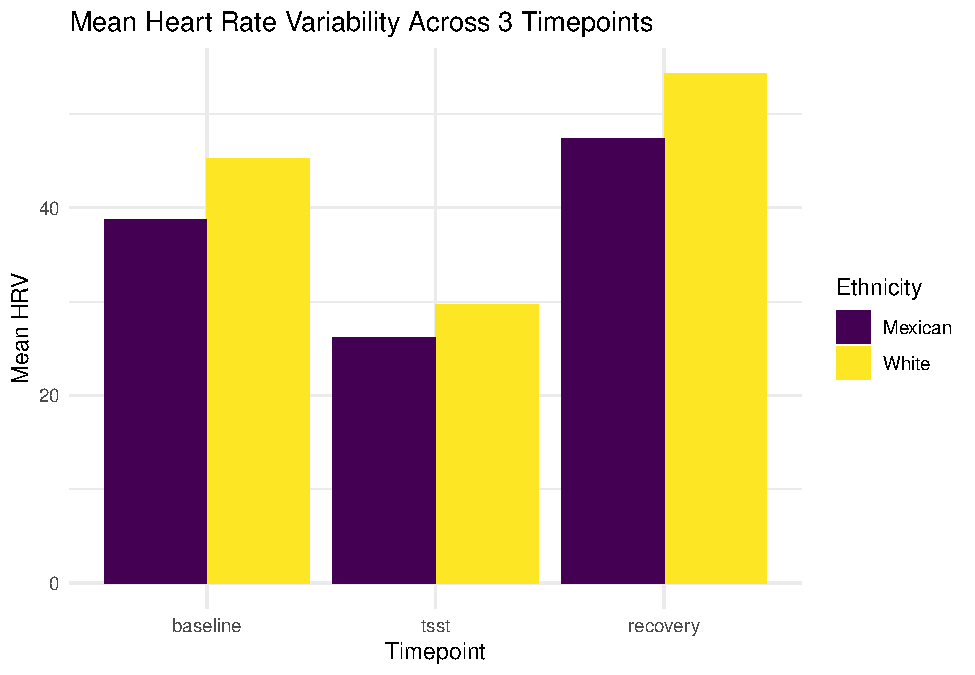
\includegraphics{PAPAJA_Final_class_project_files/figure-latex/unnamed-chunk-2-1.pdf}
\caption{\label{fig:unnamed-chunk-2}\emph{Heartrate variability by ethnicity across time points.}}
\end{figure}

\begin{figure}
\centering
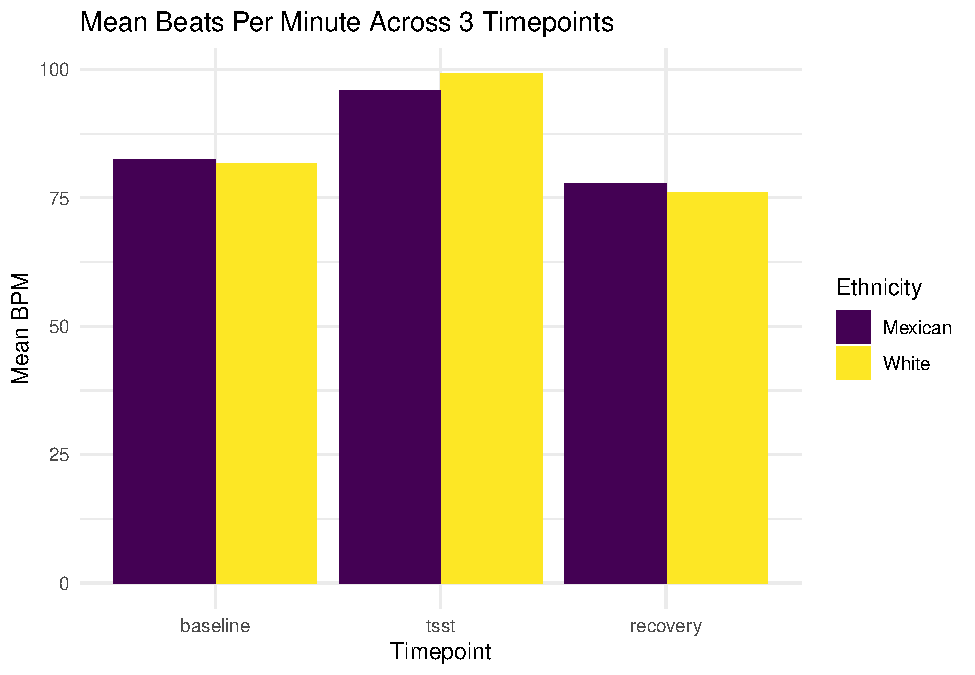
\includegraphics{PAPAJA_Final_class_project_files/figure-latex/unnamed-chunk-3-1.pdf}
\caption{\label{fig:unnamed-chunk-3}\emph{Heartrate beats per minute by ethnicity across time points.}}
\end{figure}

\hypertarget{references}{%
\section{References}\label{references}}

\begingroup
\setlength{\parindent}{-0.5in}
\setlength{\leftskip}{0.5in}

\hypertarget{refs}{}
\leavevmode\hypertarget{ref-bixler2002insomnia}{}%
Bixler, E., Vgontzas, A., Lin, H.-M., Vela-Bueno, A., \& Kales, A. (2002). Insomnia in central pennsylvania. \emph{Journal of Psychosomatic Research}, \emph{53}(1), 589--592.

\leavevmode\hypertarget{ref-buboltz2001sleep}{}%
Buboltz Jr, W. C., Brown, F., \& Soper, B. (2001). Sleep habits and patterns of college students: A preliminary study. \emph{Journal of American College Health}, \emph{50}(3), 131--135.

\leavevmode\hypertarget{ref-cohen2007_psych}{}%
Cohen, S., Janicki-Deverts, D., \& Miller, G. E. (2007). Psychological stress and disease. \emph{Jama}, \emph{298}(14), 1685--1687.

\leavevmode\hypertarget{ref-doane2015multi}{}%
Doane, L. D., Gress-Smith, J. L., \& Breitenstein, R. S. (2015). Multi-method assessments of sleep over the transition to college and the associations with depression and anxiety symptoms. \emph{Journal of Youth and Adolescence}, \emph{44}(2), 389--404.

\leavevmode\hypertarget{ref-fuligni2006daily}{}%
Fuligni, A. J., \& Hardway, C. (2006). Daily variation in adolescents' sleep, activities, and psychological well-being. \emph{Journal of Research on Adolescence}, \emph{16}(3), 353--378.

\leavevmode\hypertarget{ref-fuligni2015daily}{}%
Fuligni, A. J., Tsai, K. M., Krull, J. L., \& Gonzales, N. A. (2015). Daily concordance between parent and adolescent sleep habits. \emph{Journal of Adolescent Health}, \emph{56}(2), 244--250.

\leavevmode\hypertarget{ref-galambos2009losing}{}%
Galambos, N. L., Dalton, A. L., \& Maggs, J. L. (2009). Losing sleep over it: Daily variation in sleep quantity and quality in canadian students' first semester of university. \emph{Journal of Research on Adolescence}, \emph{19}(4), 741--761.

\leavevmode\hypertarget{ref-garde_2012_bi}{}%
Garde, A. H., Albertsen, K., Persson, R., Hansen, Å. M., \& Rugulies, R. (2012). Bi-directional associations between psychological arousal, cortisol, and sleep. \emph{Behavioral Sleep Medicine}, \emph{10}(1), 28--40.

\leavevmode\hypertarget{ref-hale2007racial}{}%
Hale, L., \& Do, D. P. (2007). Racial differences in self-reports of sleep duration in a population-based study. \emph{Sleep}, \emph{30}(9), 1096--1103.

\leavevmode\hypertarget{ref-howrey2012self}{}%
Howrey, B. T., Peek, M. K., Raji, M. A., Ray, L. A., \& Ottenbacher, K. J. (2012). Self-reported sleep characteristics and mortality in older adults of mexican origin: Results from the h ispanic e stablished p opulation for the e pidemiologic s tudy of the e lderly. \emph{Journal of the American Geriatrics Society}, \emph{60}(10), 1906--1911.

\leavevmode\hypertarget{ref-hunt2003all}{}%
Hunt, K. J., Resendez, R. G., Williams, K., Haffner, S. M., Stern, M. P., \& Hazuda, H. P. (2003). All-cause and cardiovascular mortality among mexican-american and non-hispanic white older participants in the san antonio heart study---evidence against the ``hispanic paradox''. \emph{American Journal of Epidemiology}, \emph{158}(11), 1048--1057.

\leavevmode\hypertarget{ref-jean2000sleep}{}%
Jean-Louis, G., Kripke, D. F., Ancoli-Israel, S., Klauber, M. R., \& Sepulveda, R. S. (2000). Sleep duration, illumination, and activity patterns in a population sample: Effects of gender and ethnicity. \emph{Biological Psychiatry}, \emph{47}(10), 921--927.

\leavevmode\hypertarget{ref-knutson2010sleep}{}%
Knutson, K. L. (2010). Sleep duration and cardiometabolic risk: A review of the epidemiologic evidence. \emph{Best Practice \& Research Clinical Endocrinology \& Metabolism}, \emph{24}(5), 731--743.

\leavevmode\hypertarget{ref-krueger2009sleep}{}%
Krueger, P. M., \& Friedman, E. M. (2009). Sleep duration in the united states: A cross-sectional population-based study. \emph{American Journal of Epidemiology}, \emph{169}(9), 1052--1063.

\leavevmode\hypertarget{ref-loredo2010sleep}{}%
Loredo, J. S., Soler, X., Bardwell, W., Ancoli-Israel, S., Dimsdale, J. E., \& Palinkas, L. A. (2010). Sleep health in us hispanic population. \emph{Sleep}, \emph{33}(7), 962--967.

\leavevmode\hypertarget{ref-lund2010sleep}{}%
Lund, H. G., Reider, B. D., Whiting, A. B., \& Prichard, J. R. (2010). Sleep patterns and predictors of disturbed sleep in a large population of college students. \emph{Journal of Adolescent Health}, \emph{46}(2), 124--132.

\leavevmode\hypertarget{ref-mellman_2018_SNS}{}%
Mellman, T. A., Bell, K. A., Abu-Bader, S. H., \& Kobayashi, I. (2018). Neighborhood stress and autonomic nervous system activity during sleep. \emph{Sleep}, \emph{41}(6), zsy059.

\leavevmode\hypertarget{ref-minkel2014sleep}{}%
Minkel, J., Moreta, M., Muto, J., Htaik, O., Jones, C., Basner, M., \& Dinges, D. (2014). Sleep deprivation potentiates hpa axis stress reactivity in healthy adults. \emph{Health Psychology}, \emph{33}(11), 1430.

\leavevmode\hypertarget{ref-pedraza2012sleep}{}%
Pedraza, S., Al Snih, S., Ottenbacher, K. J., Markides, K. S., \& Raji, M. A. (2012). Sleep quality and sleep problems in mexican americans aged 75 and older. \emph{Aging Clinical and Experimental Research}, \emph{24}(4), 391--397.

\leavevmode\hypertarget{ref-R-base}{}%
R Core Team. (2019). \emph{R: A language and environment for statistical computing}. Vienna, Austria: R Foundation for Statistical Computing. Retrieved from \url{https://www.R-project.org/}

\leavevmode\hypertarget{ref-ruiz2016hispanic}{}%
Ruiz, J. M., Hamann, H. A., Mehl, M. R., \& O'Connor, M.-F. (2016). The hispanic health paradox: From epidemiological phenomenon to contribution opportunities for psychological science. \emph{Group Processes \& Intergroup Relations}, \emph{19}(4), 462--476.

\leavevmode\hypertarget{ref-ruiz2018hispanic}{}%
Ruiz, J. M., Sbarra, D., \& Steffen, P. R. (2018). Hispanic ethnicity, stress psychophysiology and paradoxical health outcomes: A review with conceptual considerations and a call for research. \emph{International Journal of Psychophysiology}, \emph{131}, 24--29.

\leavevmode\hypertarget{ref-sladek2015daily}{}%
Sladek, M. R., \& Doane, L. D. (2015). Daily diary reports of social connection, objective sleep, and the cortisol awakening response during adolescents' first year of college. \emph{Journal of Youth and Adolescence}, \emph{44}(2), 298--316.

\leavevmode\hypertarget{ref-tsai2004sleep}{}%
Tsai, L.-L., \& Li, S.-P. (2004). Sleep patterns in college students: Gender and grade differences. \emph{Journal of Psychosomatic Research}, \emph{56}(2), 231--237.

\leavevmode\hypertarget{ref-yim2015experimental}{}%
Yim, I. S., Quas, J. A., Rush, E. B., Granger, D. A., \& Skoluda, N. (2015). Experimental manipulation of the trier social stress test-modified (tsst-m) to vary arousal across development. \emph{Psychoneuroendocrinology}, \emph{57}, 61--71.

\endgroup

\end{document}
